\documentclass{report}
\usepackage{fancyhdr} % Required for custom headers
\usepackage{lastpage} % Required to determine the last page for the footer
\usepackage{extramarks} % Required for headers and footers
\usepackage{graphicx} % Required to insert images
%\usepackage{lipsum} % Used for inserting dummy 'Lorem ipsum' text into the template
\usepackage{amsmath}
\usepackage{graphicx} 
%\usepackage{amsfont}
%\usepackage{amssymb}
\usepackage{float}
\usepackage{multicol}
% Margins
\topmargin=-0.5in
\evensidemargin=0in
\oddsidemargin=-0.5in
\textwidth=7.5in
\textheight=9.0in
\headsep=0.25in 


\pagestyle{fancy}

%\rhead{\textbf{Marshall's Recipes}} % Top right header
%\lhead{\textbf{Curry Stir Fry}}
%\chead{ }
%\title{Curry Stir Fry}

\begin{document}
%\vspace{8mm}
%\textbf{PRELIMINARIES:}


\bigskip

\bigskip

\begin{multicols}{2}
\textbf{Ingredients}
\begin{itemize}
\item 1 onion \quad (45 kCal/ 1 gP/ 0 gF/ 11 gC)
\item 2 lbs cubed chicken breast \newline(1496 kCal/ 280 gP/  32 gF/ 0 gC)
\item 2 cans of cream of chicken soup  \quad (650 kCal/ 10 gP/ 45 gF/ 18 gC)
\item 1 lb baby carrots \quad (186 kCal / 4 gP / 0 gF / 45 gC)
\item 3 russet potatoes (medium/medium large) \quad (504 kCal/ 15 gP/ 0 gF/ 111 gC)
\item 1 Jar of green chile (I use santa fe hot)\newline  (90 kCal /8 gP/ 0 gF/ 48 gC)
\item 1 can of corn (with water) \quad (280 kCal/ 7 gP/ 5 gF/ 32 gC)
\item $\sim 5$ cloves of garlic (minced) (65 kCal /3 gP/ 0 gF/ 15 gC) 
\item 4-5 cups of water (enough to fill $\frac{1}{4}$ inch from rim of crock pot.)
\item (optional: 1 slice of colby jack cheese on top, not included in totals below) \newline (80 kCal / 5 gP/ 6 gF/ 0 gC)
\item 6-7 cubes of chicken bullion 
\item 2 tsp. salt
\item 1 tsp. black pepper
\item 3 bay leaves



\end{itemize}


\columnbreak
\textbf{Procedure:}
\medskip


\begin{enumerate}
\item \textbf{\textit{Note:}}This is a MASSIVE recipe. This will fill an 8-quart slow cooker to the brim. 
\item Dice onion, cube potatoes, and chop carrots into bite size pieces. Add to crock pot. Add canned items, and freeze the remaining green chile.  


\medskip
\item Cube chicken and add garlic and bullion. Add salt and black pepper and mix thoroughly. Set on low for 8-9 hours or high for 5-6 hours. 
  
\begin{table}[H]
    \centering
    \caption{Macro totals}
    \label{tab:table1}
    \begin{tabular}{c|c|c|c} % <-- Alignments: 1st column left, 2nd middle and 3rd right, with vertical lines in between
      \textbf{Calories} & \textbf{Protein} & \textbf{Fat} & \textbf{Carbs}\\
      \hline
      3,316 kCal & 328 g & 82 g & 295 g\\
    \end{tabular}
\end{table}

\end{enumerate}
\end{multicols}



%\begin{center}
%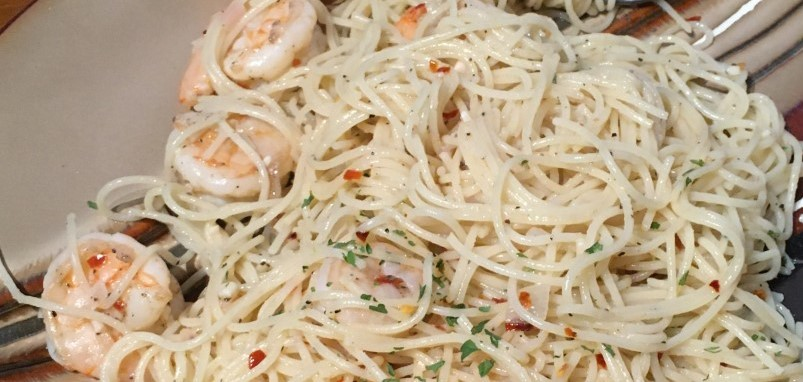
\includegraphics[scale=0.65]{Pasta/Shrimp Scampi/Shrimp Scampi.jpg}
%\end{center}


\end{document}